% Copyright (c) 2009-2015 by the University of Waikato, Hamilton, NZ.
% This work is made available under the terms of the 
% Creative Commons Attribution-ShareAlike 4.0 license,
% http://creativecommons.org/licenses/by-sa/4.0/.
%
% Version: $Revision: 3363 $

\documentclass[a4paper]{book}

\usepackage{wrapfig}
\usepackage{graphicx}
\usepackage{hyperref}
\usepackage{multirow}
\usepackage{scalefnt}
\usepackage{tikz}
\usepackage{varwidth}

% watermark -- for draft stage
%\usepackage[firstpage]{draftwatermark}
%\SetWatermarkLightness{0.9}
%\SetWatermarkScale{5}

\hyphenation{ImageMagick}
\hyphenation{ImageJ}

% Copyright (c) 2009 by the University of Waikato, Hamilton, NZ. 
% This work is made available under the terms of the 
% Creative Commons Attribution-ShareAlike 4.0 license,
% http://creativecommons.org/licenses/by-sa/4.0/.
%
% Version: $Revision: 2916 $

\newenvironment{tight_itemize}{
\begin{itemize}
  \setlength{\itemsep}{1pt}
  \setlength{\parskip}{0pt}
  \setlength{\parsep}{0pt}}{\end{itemize}
}

\newenvironment{tight_enumerate}{
\begin{enumerate}
  \setlength{\itemsep}{1pt}
  \setlength{\parskip}{0pt}
  \setlength{\parsep}{0pt}}{\end{enumerate}
}

% if you just need a simple heading
% Usage:
%   \heading{the text of the heading}
\newcommand{\heading}[1]{
  \vspace{0.3cm} \noindent \textbf{#1} \newline
}

\newcommand{\icon}[1]{\tikz[baseline=-3pt]\node[inner sep=0pt,outer sep=0pt]{\includegraphics[height=1.1em]{#1}};}


\title{
  \textbf{ADAMS} \\
  {\Large \textbf{A}dvanced \textbf{D}ata mining \textbf{A}nd \textbf{M}achine
  learning \textbf{S}ystem} \\
  {\Large Module: adams-imaging-imagemagick} \\
  \vspace{1cm}
  
\includegraphics[width=2cm]{images/imaging-imagemagick-module.png} \\
}
\author{
  Peter Reutemann
}

\setcounter{secnumdepth}{3}
\setcounter{tocdepth}{3}

\begin{document}

\begin{titlepage}
\maketitle

\thispagestyle{empty}
\center
\begin{table}[b]
	\begin{tabular}{c l l}
		\parbox[c][2cm]{2cm}{\copyright 2009-2015} &
		\parbox[c][2cm]{5cm}{
\includegraphics[width=5cm]{images/coat_of_arms.pdf}} \\
	\end{tabular}
	
\includegraphics[width=12cm]{images/cc.png} \\
\end{table}

\end{titlepage}

\tableofcontents
\listoffigures
%\listoftables


%%%%%%%%%%%%%%%%%%%%%%%%%%%%%%%%%%%
\chapter{ImageMagick}
ImageMagick$\textsuperscript{\textregistered}$ is a software suite to create,
edit, compose, or convert bitmap images (\cite{imagemagick}). On Windows, in order to
process images with ImageMagick, you need to set the \texttt{IM\_TOOLPATH} 
environment variable, pointing to the installation. Similar, for dcraw, you 
need to defined the \texttt{DCRAW\_TOOLPATH} variable and, for ufraw, the
\texttt{UFRAW\_TOOLPATH} one.

The following ImageMagick actors available:
\begin{tight_itemize}
	\item \texttt{transformer.ImageMagickOperation} -- performs the ImageMagick
	(convert, dcraw, ufraw) operations that the user selected from the class
	hierarchy.
	\item \texttt{transformer.ImageMagickTransformer} -- performs any ImageMagick
	command on the incoming image that the \texttt{convert} tool\footnote{\url{http://www.imagemagick.org/script/convert.php}{}} supports and
	outputs another image again.
\end{tight_itemize}

Reading and writing images are done using the \textit{ImageReader} transformer
and \textit{ImageWriter} sink:
\begin{tight_itemize}
	\item \texttt{ImageReader} -- use the \textit{ImageMagickImageReader} or \textit{UIfrawImageReader}
	\item \texttt{ImageWriter} -- use the \textit{ImageMagickImageWriter}
\end{tight_itemize}

There is no separate transformer for generating a WEKA instance, since the
ImageMagick actors process and output \texttt{BufferedImageContainer} objects as
well, just like the JAI actors. You can use the \texttt{BufferedImageFeatureGenerator} for
generating WEKA output.

The example flow\footnote{adams-imaging-imagemagick\_script.flow} in Figure
\ref{imagemagick-resize-flow} loads a single photo from disk and then uses
ImageMagick to resize it to 90 by 90 pixels and scaling it by 200\% (see
\ref{imagemagick-resize-script}). Finally, the modified image is displayed in
the image viewer.

\begin{figure}[htb]
  \centering
  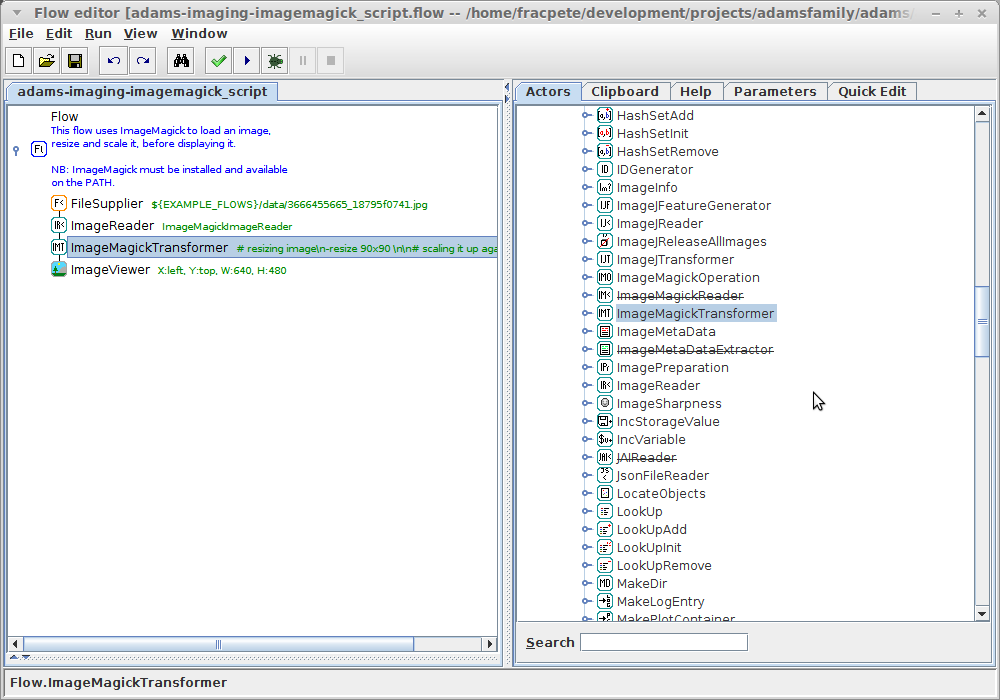
\includegraphics[width=10.0cm]{images/imagemagick-resize-flow.png}
  \caption{ImageMagick flow for processing (resizing) a single image.}
  \label{imagemagick-resize-flow}
\end{figure}

\begin{figure}[htb]
  \begin{center}
  \begin{varwidth}{\textwidth}
\begin{verbatim}
# resizing image
-resize 90x90
# scaling it up again
-scale 200%
\end{verbatim}
  \end{varwidth}
  \end{center}
  \caption{ImageMagick commands to resizing.}
  \label{imagemagick-resize-script}
\end{figure}

\begin{figure}[htb]
  \begin{minipage}[b]{0.48\linewidth}
  \centering
  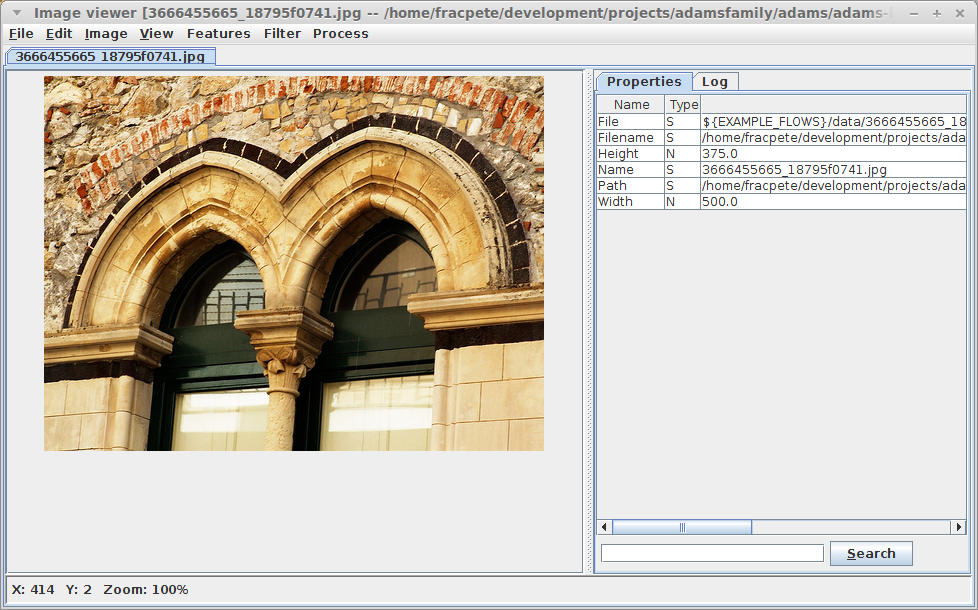
\includegraphics[height=3.8cm]{images/imagemagick-resize-original.png}
  \caption{The original image.}
  \label{imagemagick-resize-original}
  \end{minipage}%
  \begin{minipage}[b]{0.48\linewidth}
  \centering
  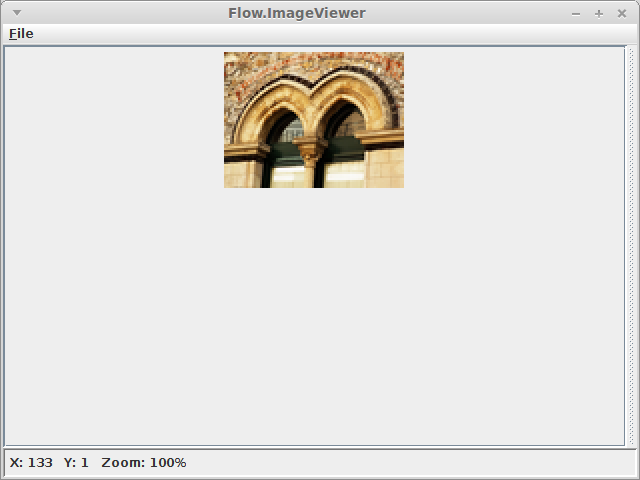
\includegraphics[height=3.8cm]{images/imagemagick-resize-output.png}
  \caption{The resized image.}
  \label{imagemagick-resize-output}
  \end{minipage}
\end{figure}

%%%%%%%%%%%%%%%%%%%%%%%%%%%%%%%%%%%
% Copyright (c) 2009-2012 by the University of Waikato, Hamilton, NZ. 
% This work is made available under the terms of the 
% Creative Commons Attribution-ShareAlike 4.0 license,
% http://creativecommons.org/licenses/by-sa/4.0/.
%
% Version: $Revision: 3353 $

\begin{thebibliography}{999}
	% to make the bibliography appear in the TOC
	\addcontentsline{toc}{chapter}{Bibliography}

    % references
	\bibitem{adams}
		\textit{ADAMS} -- Advanced Data mining and Machine learning System \\
		\url{https://adams.cms.waikato.ac.nz/}{}

	\bibitem{imagemagick}
		\textit{ImageMagick} -- Software suite to Convert, Edit, and Compose Images \\
		\url{http://www.imagemagick.org/}{}

\end{thebibliography}


\end{document}
